\chapter{Modelo de míneria de datos genómicos}

\section{Introducción}

La necesidad de comprender los procesos biologícos que están implicados en las distintas enfermedades, a partir de la gran cantidad de datos biológicos que hay disponibles como las secuencias genómicas, los microarreglos, las interacciones proteicas, las imágenes biomedicas entre otros. Además la rápida adopción de las historias clínicas electrónicas proporciona una oportunidad de realizar investigaciones a gran escala. Por lo tanto las técnicas de minería de datos para el descubrimiento de conocimiento a partir de la obtención de información de diferentes fuentes son cada vez mas importantes en la biología y en el el cuidado de la salud \cite{Wang2017}.\\

Algunos de los impedimentos para la minería de datos a gran escala en datos genómicos son la disponibilidad de los datos, el tamaño de los datos y los algoritmos y modelos para la integración, algunos de los desafíos son la manipulación de datos de gran tamaño. Casi todos los tipos de datos biológicos presentan una acumulación exponencial, donde la minería de datos genómicos a gran escala es una necesidad ya que estos son los que presentan un aumento mayor gracias a las tecnologías de secuenciación (NGS) \cite{Huttenhower2010}.\\

El mayor reto de la minería de datos genómicos esta en la extracción de información relevante de grandes cantidades de datos clínicos y transformarlos en conocimiento, los mayores retos están en: a) La recolección de los datos clínicos y genómicos, b) recuperación de información relevante de datos y c) extracción de nuevos conocimientos de la información \cite{Farid2016}. \\  

Para los datos genómicos se han propuesto la utilización de paneles a partir de secuenciación de exomas,donde se hace el preprocesamiento,selección de características, selección y aplicación de algoritmos de minería finalmente para el descubrimiento del conocimiento a partir de datos genómicos \cite{Farid2016}. \\

\section{Metodología}

Se diseño un modelo de minería que se realizo como muestra la figura \ref{fig:mineria}:

\begin{figure}[H]
	\centering
	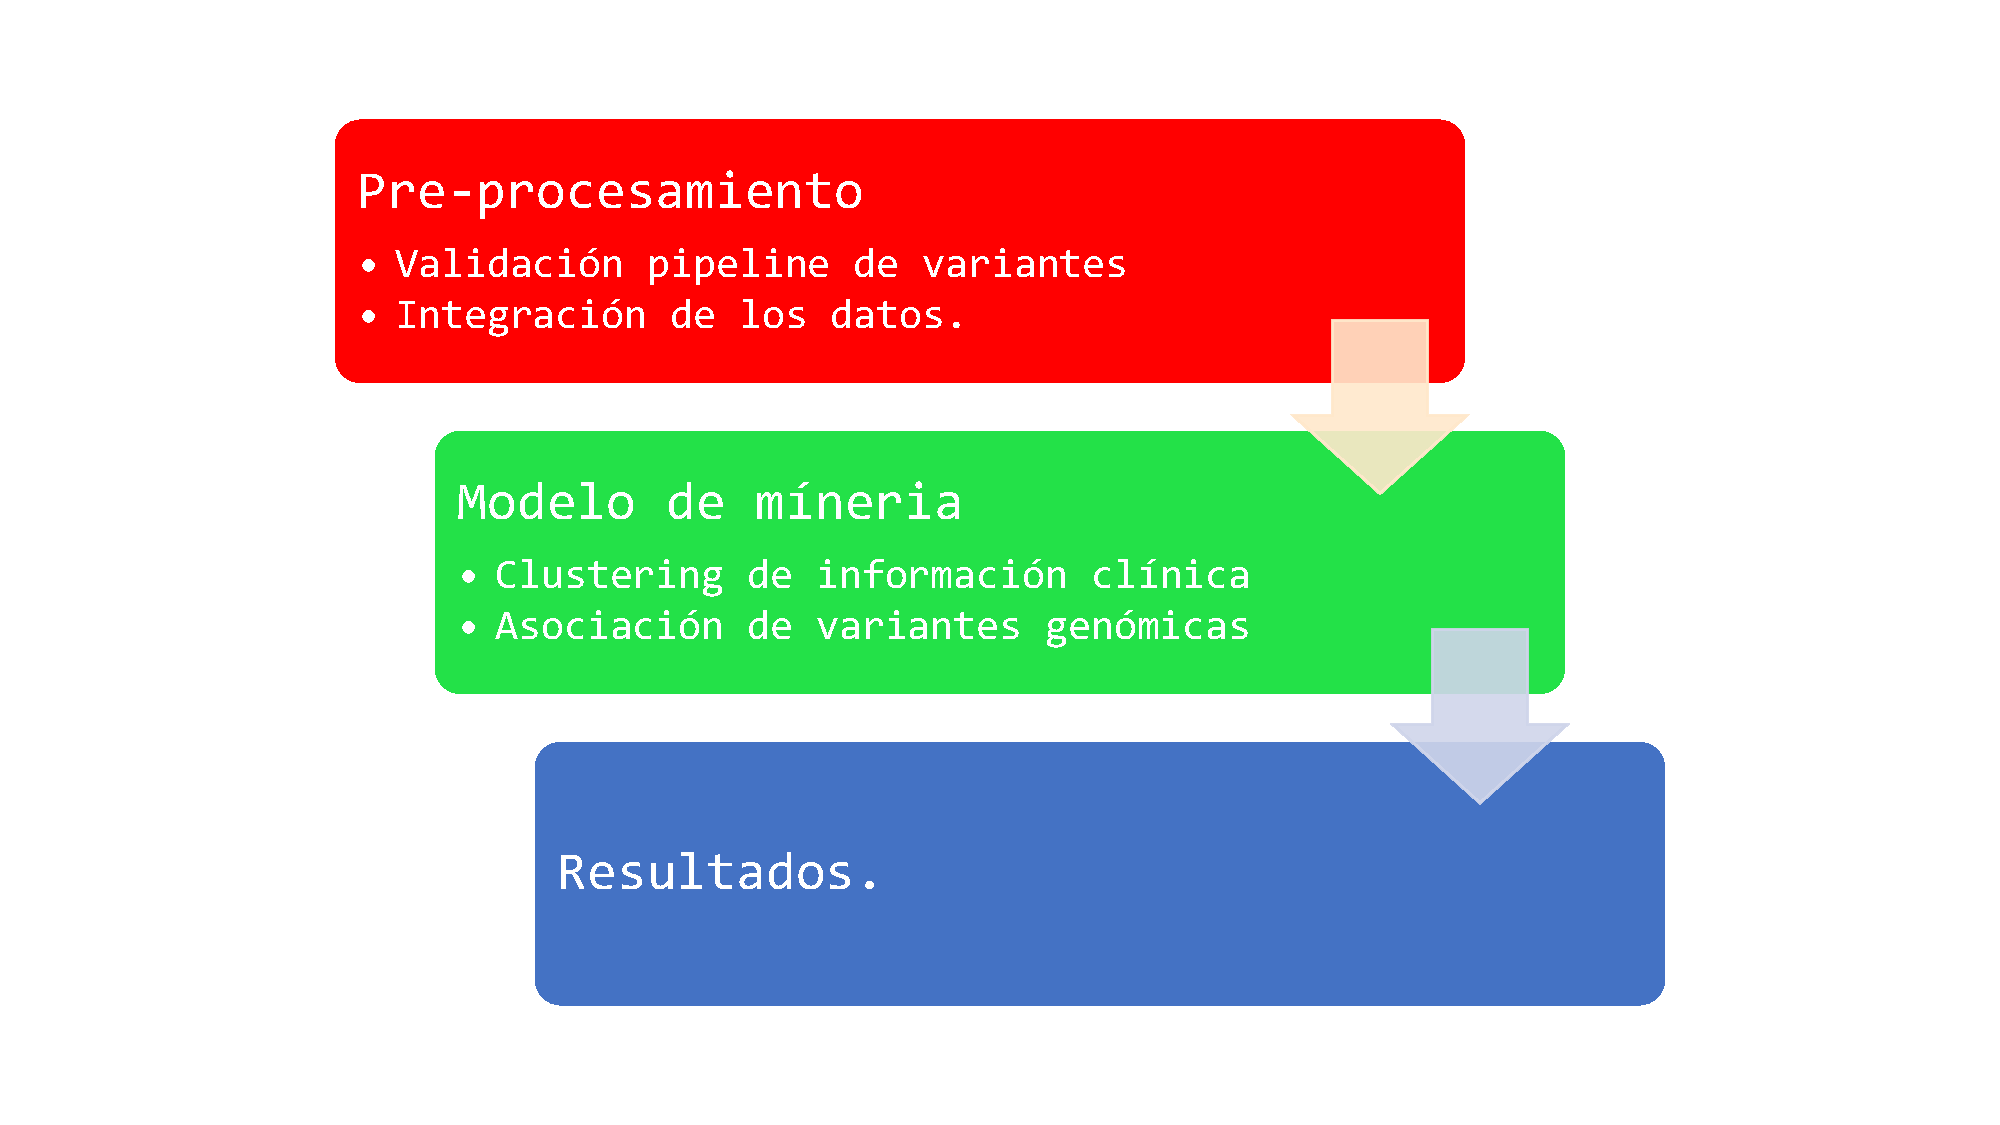
\includegraphics[width=0.5\textwidth]{Kap4/pipelinemineria}
	\caption{Proceso de minería} \label{fig:mineria}
\end{figure} 

Después de la implementación se realizo un preprocesamiento que fue la limpieza de stop words en español, remoción de tildes y ñ, y reemplazo de palabras sinónimas dentro de las historias clínicas. Se realizo la obtención de la frecuencia de términos con la librería nltk de python y el tfidf tm de R. Una vez realizado este procedimiento se realizo un clustering con el algoritmo kmeans ++  con los parametros por defecto implementado en python 2.7.13 de la librería sklearn de python, previamente se calculo el número de k con el error cuadrático y el valor de silueta también implementado en la librería de sklearn de python y los gráficos fueron realizados con la librerías pandas y matplolib.
 
\section{Resultados}

Los resultados que se obtuvieron fueron que las palabras más frecuentes fueron seno, cancer, sindrome, sospecha y años. La figura \ref{fig:sin} muestra la frecuencia de palabras que se obtuvieron dentro de la base de datos.

\begin{figure}[H]
	\centering
	\subfigure[Nube de palabras]{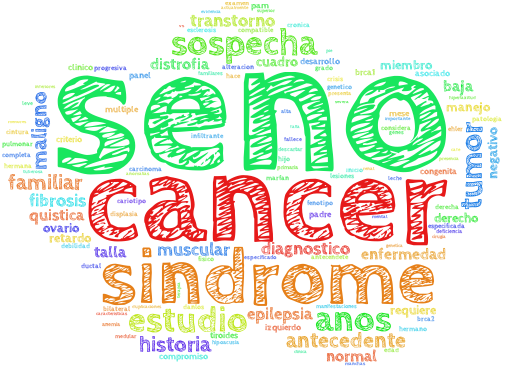
\includegraphics[width=60mm]{Kap4/sin_stop}}
	\subfigure[Frecuencia de términos]{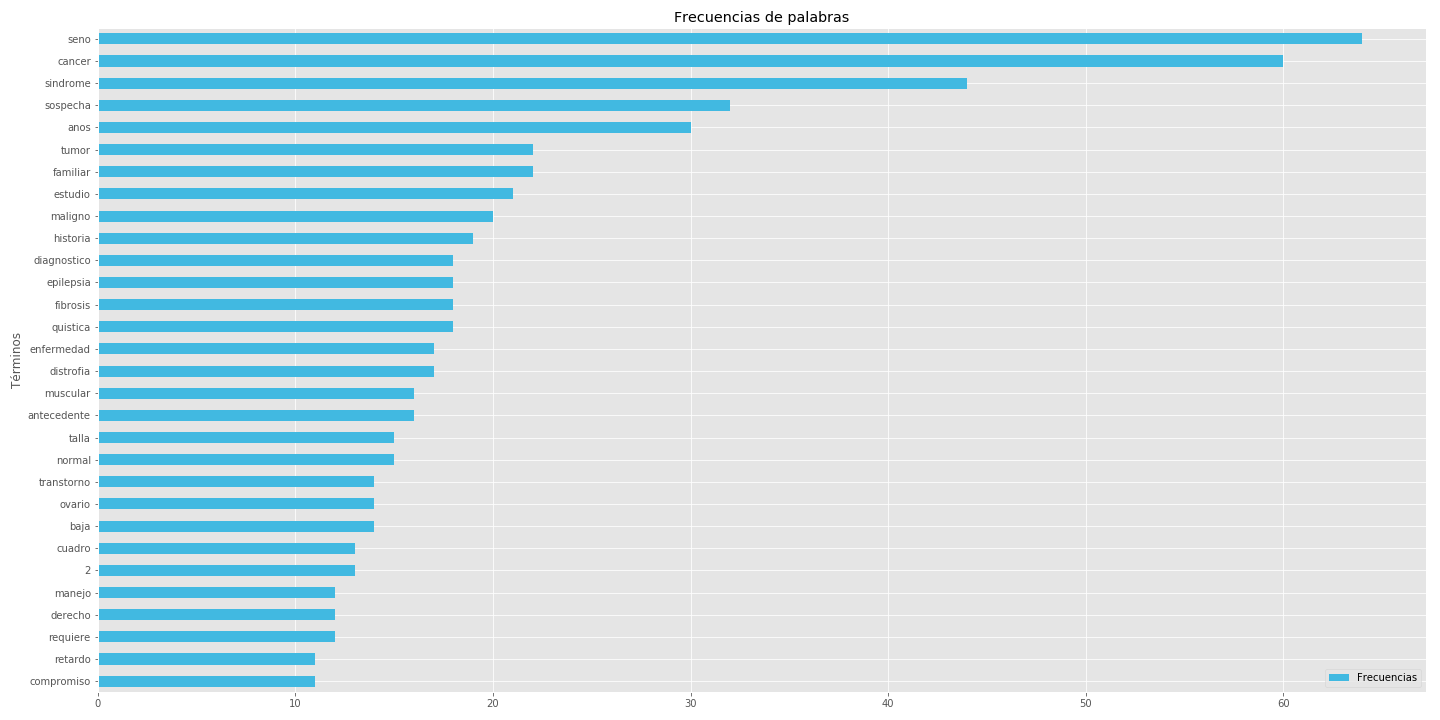
\includegraphics[width=60mm]{Kap4/frecuecias}}
	\caption{Frecuencias sin stop words y palabras sinónimas} \label{fig:sin}
\end{figure} 

La figura \ref{fig:IDFTF} representa la matriz IDF-TF de las palabras que se encuentran dentro de la base de datos.  

\begin{figure}[H] 
	\centering
	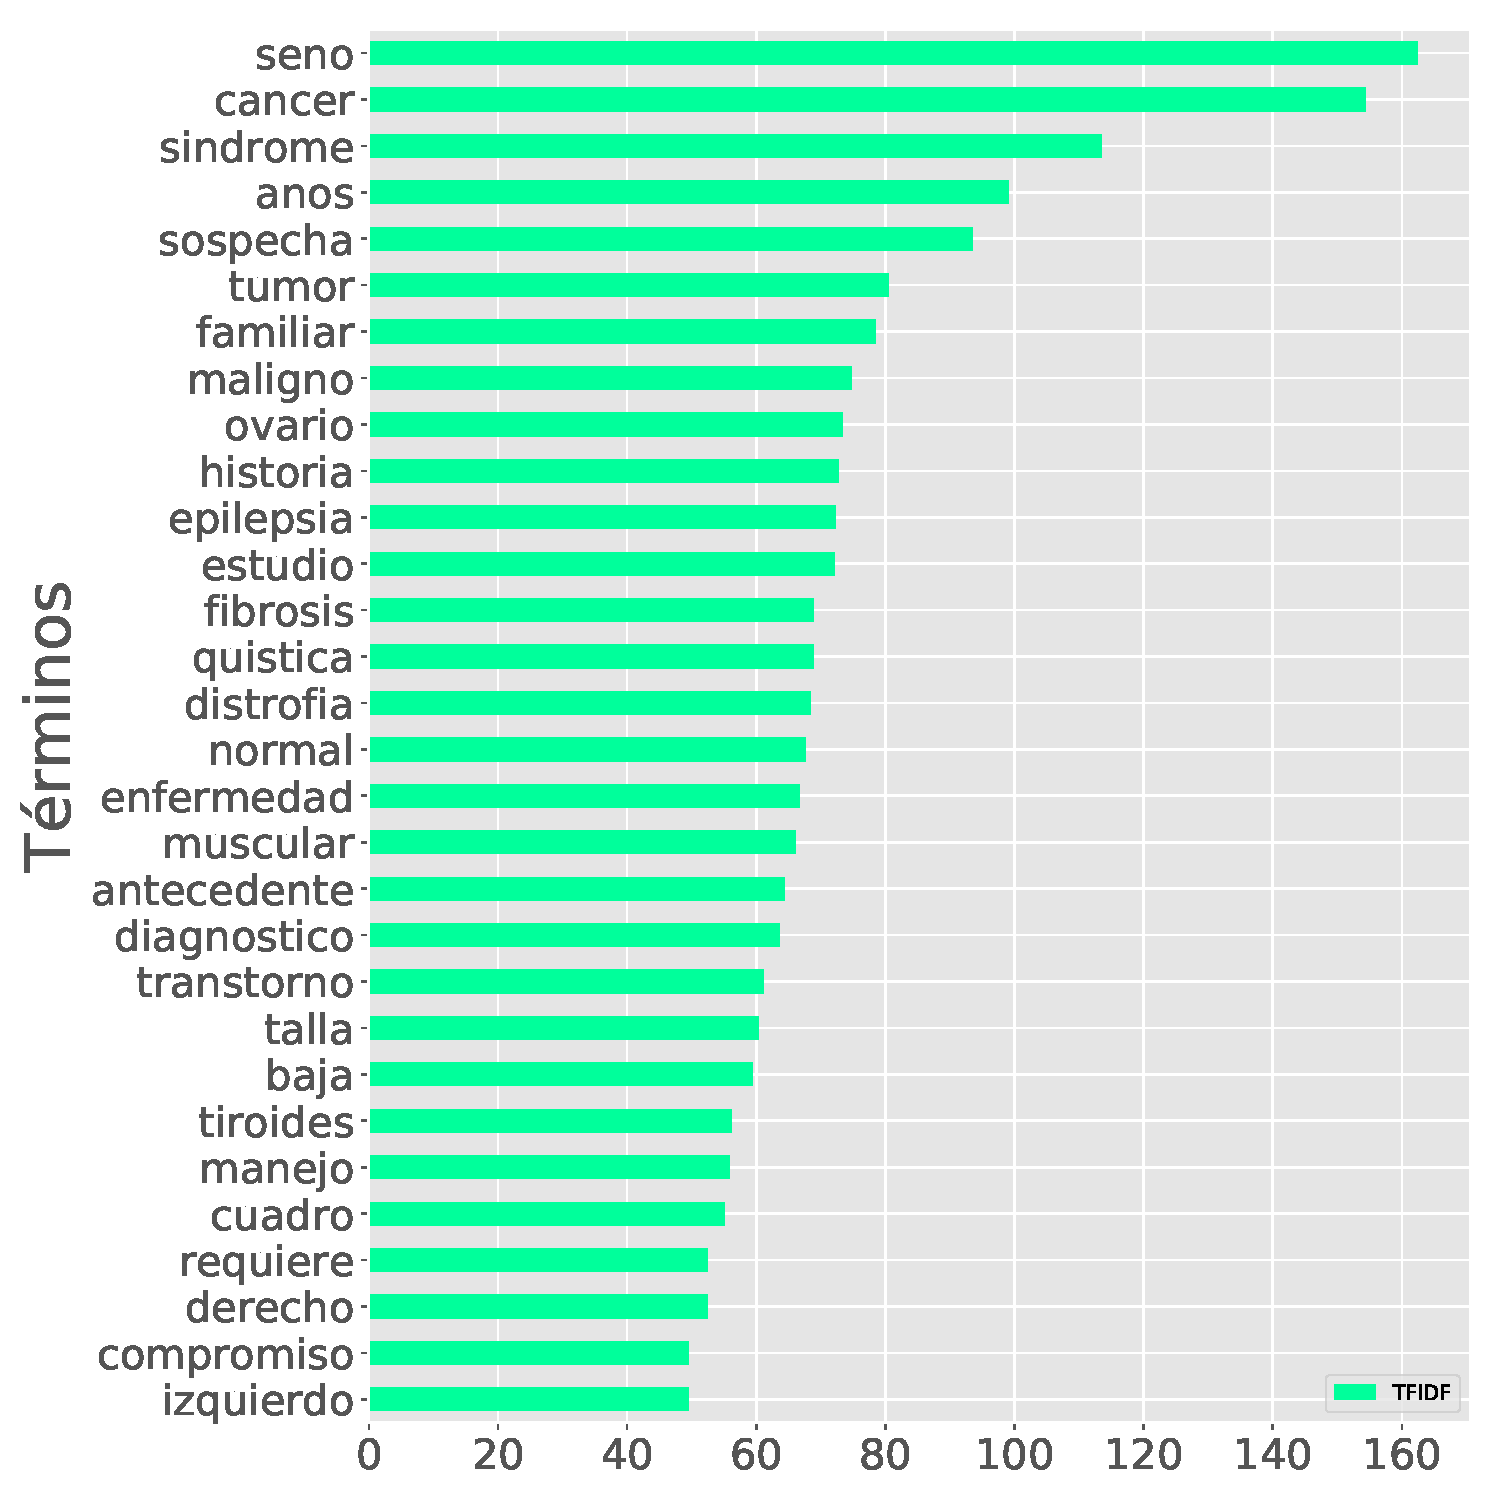
\includegraphics[width=0.8\textwidth]{Kap4/TFIDF1}
	\caption{TFIDF} 
	\label{fig:IDFTF}
\end{figure}

Una vez realizada la selección de el número optimo de K se ejecuto el algoritmo kmeans obteniendo cinco clusters:

\begin{figure}[H] 
	\centering
	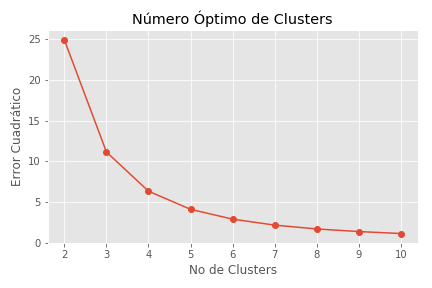
\includegraphics[width=0.5\textwidth]{Kap4/Clusters}
	\caption{Número optimo de clusters} 
	\label{fig:Clusters}
\end{figure}


\begin{figure}[H] 
	\centering
	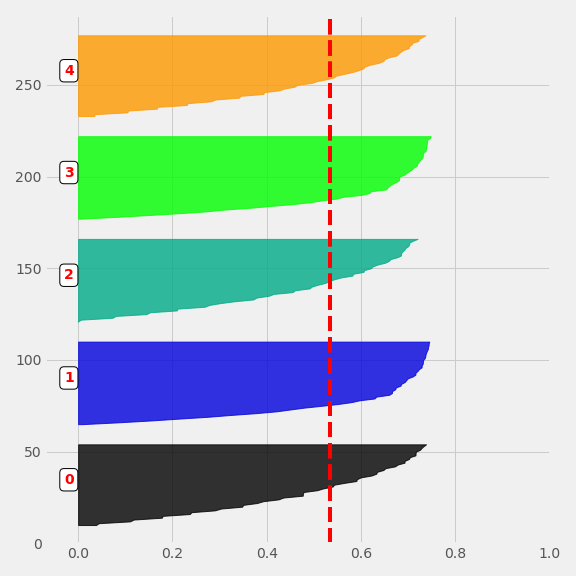
\includegraphics[width=0.5\textwidth]{Kap4/S}
	\caption{Valor Silueta de cada cluster} 
	\label{fig:S}
\end{figure}



Donde ....

\begin{figure}[H]
	\centering
	\subfigure[Nube de palabras]{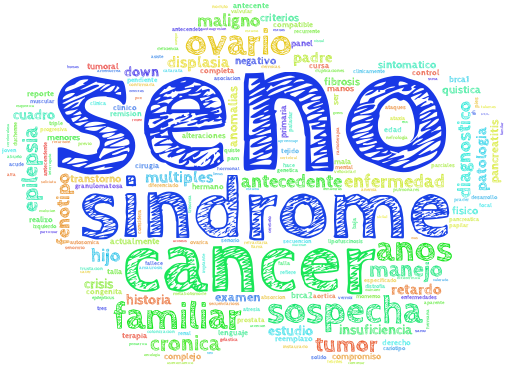
\includegraphics[width=60mm]{Kap4/cluster1}}
	\subfigure[Rango de edad en decadas]{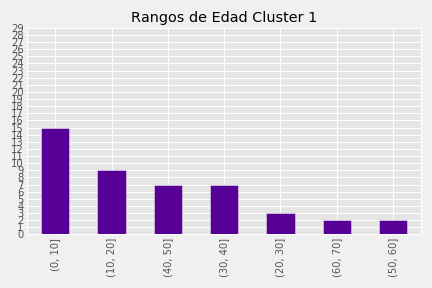
\includegraphics[width=60mm]{Kap4/edadcluster1}}
	\subfigure[Género]{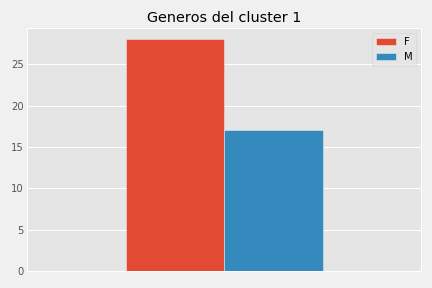
\includegraphics[width=60mm]{Kap4/Cluster1G}}
	\caption{Cluster 1} \label{fig:c1}
\end{figure}




La figura \ref{fig:c1} representa el clúster 1 con la información clínica que presenta en (a) tenemos la frecuencia de palabras, siendo seno,sindrome y cancer son las palabras más frecuentes, junto con ovario y familiar.


\begin{figure}[H]
	\centering
	\subfigure[Nube de palabras]{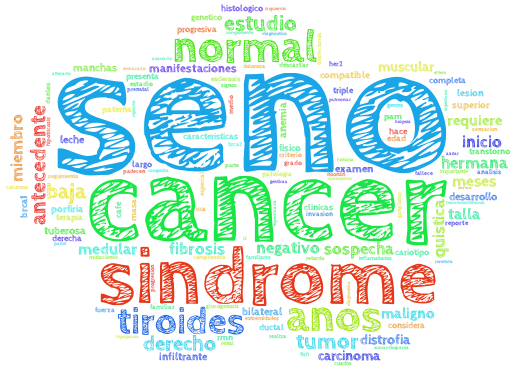
\includegraphics[width=60mm]{Kap4/cluster2}}
	\subfigure[Rango de edad en decadas]{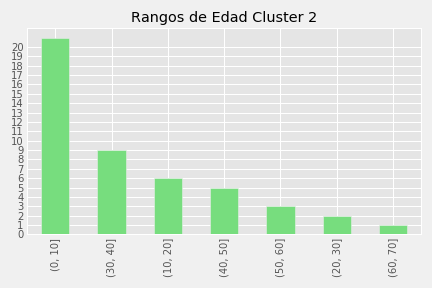
\includegraphics[width=60mm]{Kap4/edadcluster2}}
	\subfigure[Género]{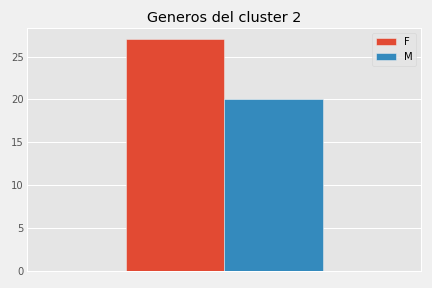
\includegraphics[width=60mm]{Kap4/Cluster2G}}
	\caption{Cluster 2} \label{fig:c2}
\end{figure}

% Please add the following required packages to your document preamble:
% \usepackage{booktabs}
% Please add the following required packages to your document preamble:
% \usepackage{booktabs}
\begin{table}[]
	\centering
	\caption{My caption}
	\label{my-label}
	\begin{tabular}{@{}|c|c|@{}}
		\toprule
		Rango de Edad & No. de pacientes . \\ \midrule
		0-10          & 15                 \\ \midrule
		10-20         & 9                  \\ \midrule
		20-30         & 3                  \\ \midrule
		30-40         & 7                  \\ \midrule
		40-50         & 7                  \\ \midrule
		50-60         & 2                  \\ \midrule
		60-70         & 2                  \\ \midrule
		Total         & 45                 \\ \bottomrule
	\end{tabular}
\end{table}

donde...

\begin{figure}[H]
	\centering
	\subfigure[Nube de palabras]{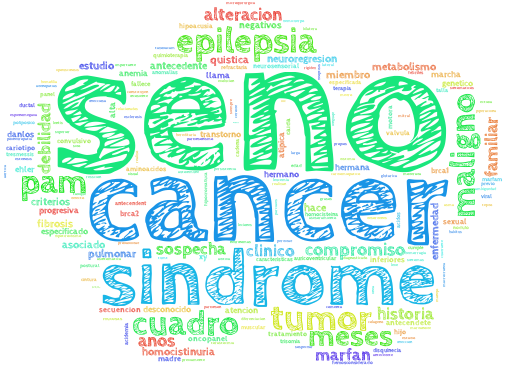
\includegraphics[width=60mm]{Kap4/cluster3}}
	\subfigure[Rango de edad en decadas]{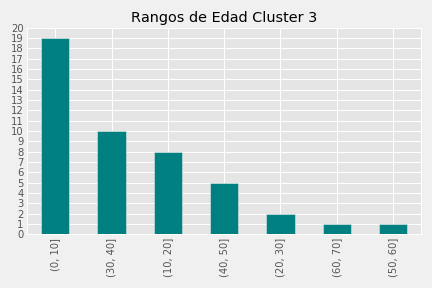
\includegraphics[width=60mm]{Kap4/edadcluster3}}
	\subfigure[Género]{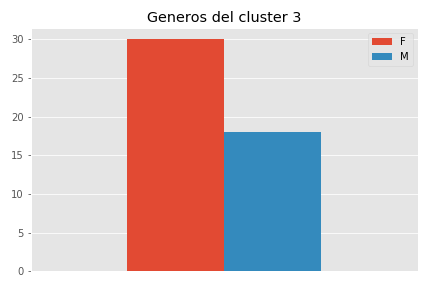
\includegraphics[width=60mm]{Kap4/Cluster3G}}
	\caption{Cluster 3} \label{fig:c3}
\end{figure}

Donde ...

\begin{figure}[H]
	\centering
	\subfigure[Nube de palabras]{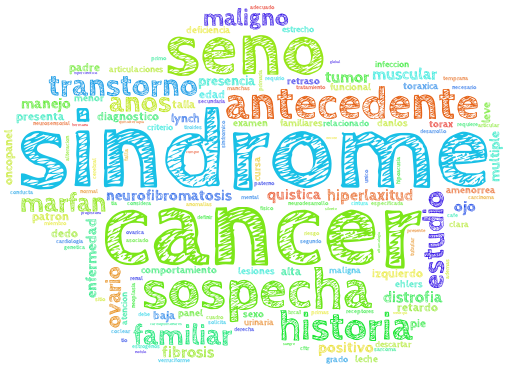
\includegraphics[width=60mm]{Kap4/cluster4}}
	\subfigure[Rango de edad en decadas]{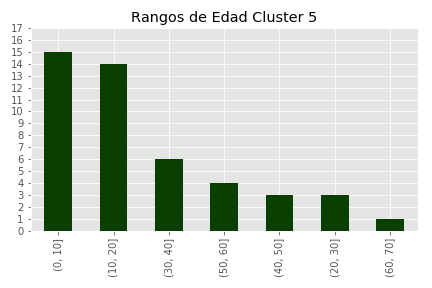
\includegraphics[width=60mm]{Kap4/edadcluster4}}
	\subfigure[Género]{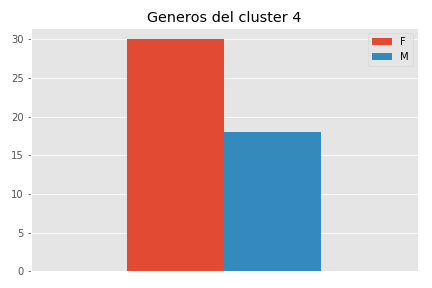
\includegraphics[width=60mm]{Kap4/Cluster4G}}
	\caption{Cluster 4} \label{fig:c4}
\end{figure}

Donde 

\begin{figure}[H]
	\centering
	\subfigure[Nube de palabras]{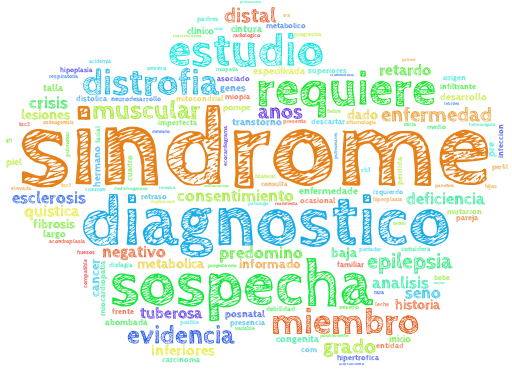
\includegraphics[width=60mm]{Kap4/cluster5}}
	\subfigure[Rango de edad en decadas]{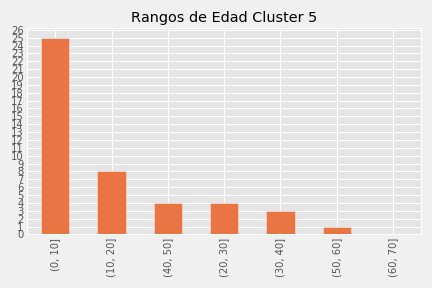
\includegraphics[width=60mm]{Kap4/edadcluster5}}
	\subfigure[Género]{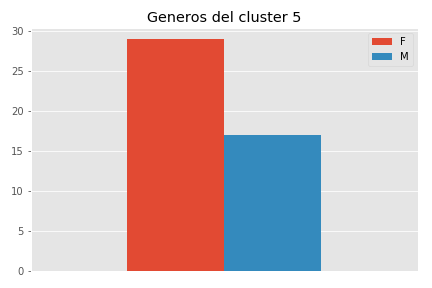
\includegraphics[width=60mm]{Kap4/Cluster5G}}
	\caption{Cluster 5} \label{fig:c5}
\end{figure}
